\documentclass[a4paper,11pt]{report}

\usepackage{fullpage}
\usepackage{amsmath}
\usepackage{bussproofs}
\usepackage{color}
\usepackage{hyperref}
\usepackage{placeins}
\usepackage{csquotes}

\usepackage{etoolbox}
\usepackage[T1]{fontenc}
\usepackage[english]{babel}
\usepackage{array}
\usepackage{graphicx}

\usepackage[
    backend=biber,
    style=alphabetic,
    sortlocale=en_GB,
    natbib=true,
    url=false,
    doi=true,
    eprint=false,
    citestyle=alphabetic-verb
]{biblatex}


% % Page style
% \usepackage{fancyhdr}

% \setlength{\headheight}{17pt}
% \pagestyle{fancy}

% % Standard pages (inside chapters)
% \fancyhf{}
% \renewcommand{\headrulewidth}{0.4pt}
% \renewcommand{\footrulewidth}{0pt}
% \fancyheadoffset{0cm}

% \fancyhead[OR]{\bfseries \nouppercase{\rightmark}}
% \fancyhead[EL]{\bfseries \nouppercase{\leftmark}}
% \fancyfoot[EL,OR]{\thepage}

%%%%%%%%%%%%%%%%%%%%%%%%%%%%%%%%%%%%%%%%%%%%%%%%%%%%%%%%%
% Minted
%%%%%%%%%%%%%%%%%%%%%%%%%%%%%%%%%%%%%%%%%%%%%%%%%%%%%%%%%

\usepackage[cache=false]{minted}
\usemintedstyle{tango}

%%%%%%%%%% C
\newmintinline{c}{
    fontsize=\small,
    breaklines=true
}

\newminted{c}{
    frame=single,
    framesep=2mm,
    fontsize=\scriptsize,
    mathescape
}

\newminted[ccodeline]{c}{
    frame=single,
    framesep=2mm,
    fontsize=\scriptsize,
    mathescape,
    linenos
}


%%%%%%%%% CMAKE
\newminted{cmake}{
    frame=single,
    framesep=2mm,
    fontsize=\scriptsize,
    mathescape,
    linenos,
    breaklines=true
}

% End minted
%%%%%%%%%%%%%%%%%%%%%%%%%%%%%%%%%%%%%%%%%%%%%%%%%%%%%%%%%

\setlength{\parindent}{0pt}

\bibliography{bibliography}

\begin{document}
    \begin{center}
        \Large{
            Operating Systems\\
            Spring 2018
        }

        \noindent\makebox[\linewidth]{\rule{\linewidth}{0.4pt}}
        Operating Systems Project
        \noindent\makebox[\linewidth]{\rule{\linewidth}{0.4pt}}

        \begin{flushleft}
            Professor : Philippe Cudre-Mauroux

            Assistant : Ines Arous
        \end{flushleft}

        \noindent\makebox[\linewidth]{\rule{\linewidth}{0.4pt}}

        Submitted by Groupe 4: Sylvain Julmy, Michael Papinutto, Sami Veillard

        \noindent\makebox[\linewidth]{\rule{\textwidth}{1pt}}
        \vspace*{0.8cm}
        \today

    \end{center}

    \newpage

    \section*{Introduction}
    For this project, we had to implement a multi-threaded client-server system using TCP sockets.
    This system had abilities to write keys with values, read values providing a key, simultaneous safe access of the readers and the writers.
    This system was subsequently tested using an automated testing in form of a bash script and text files of commands.
    One of the problem in designing such system is related to the database structure.
    Indeed, we can increase memory required but not time as this would impact User Experience.
    Hence, we tend to choose faster algorithm.
    Indeed, looking at applications usage revealed that sets are used in the following way: 90\% of calls are contains(),
    9\% are add() and 1\% are remove().
    In this project, we selected a hash set for these reasons.
    Eventhough this system might require more memory ressources and was rather complicated to implement, it was found to be efficient and powerful according to our test.


    \section*{Chosen approach}

    We had to take care of various aspect when choosing the data structure to
    store the key-value entry : maximal number of entry stored in the database,
    extension of the data structure, number of simultaneous access on the server and
    how to synchronize the threads.

    A lock-free hash-set data structure offers solutions to all of those challenges without blocking threads using mutex or semaphores.
    We have implements our own data structure in C based on the one created by
    Herlihy in \cite{Herlihy2006} in Java.

    More Specifically, we used a reversed split-ordering hash set.
    A bucket is linked to a stack.
    As the list grow supplemental buckets references are added so that no object is ever too far from the start of a bucket, \textit{i.e.}, the bucket size is keep small.
    This implementation ensures that when an item is put in the stack, it will not be move.
    However, to do so, items have to be put in the stack using a recursive-split order.
    Moreover, to avoid problems occuring when deleting node referenced by a bucket, a sentinel node is added at the beginning of each bucket.
    This special type of buckets are never deleted (see \ref{fig:Fig1}).

    \begin{figure}[h]
        \centering
            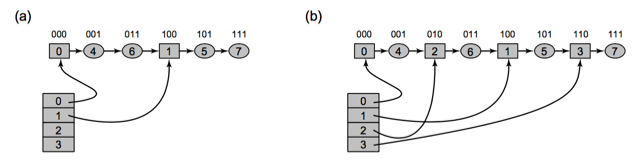
\includegraphics{hashsetFig1}
        \caption{Scheme of the recursive nature of the split ordering.
        The split order can be seen in binary words above buckets.
        Sentinel buckets are represented by square whereas ovals are normal buckets.
        (a) Shows a split-ordering including two buckets. The buckets are linked to a stack.
        (b) Shows how buckets are split in two part after the capacity of the table grows from 2 to 4.}
        \label{fig:Fig1}
    \end{figure}

    When inserting a new key in this data structure, the table is grown incrementally.
    As buckets are in a linked list ordered using split-ordering, the table resizing mechanism is independant to the threshold that decide when resizing.
    As the sets grows more of the array will be use. Hence, when adding new values to a not yet initialized bucket that should have be initialized according to the current table capacity, it will be initialized (see \ref{fig:Fig2}).


    \begin{figure}[h]
        \centering
            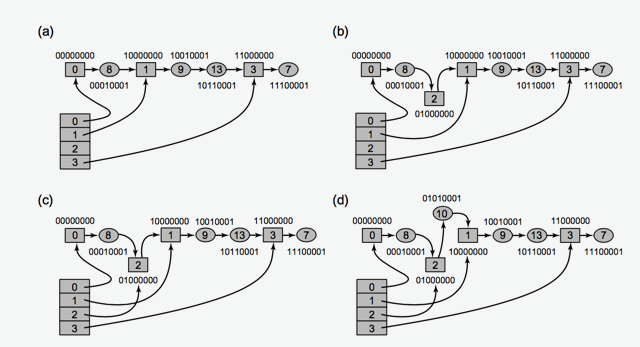
\includegraphics{hashsetFig2}
        \caption{Scheme of the procedure that add the key 10 to the lock-free hash set.
        As above, split-order key values are expressed in binary above buckets (here 8 bits words).
        (a) Buckets 0, 1 and 3 but bucket 2 is not.
        (b) An object with hash value of 10 is inserted to the set. This cause bucket 2 to be initialized and to add a new sentinel is inserted with split-order key 2.
        (c) Bucket 2 is affiliated with a new sentinel.
        (d) Finally, the split-order ordinary key 10 is added to bucket 2.}
        \label{fig:Fig2}
    \end{figure}

    In summary, our chosen approach implements a split-ordered hash set which is an array of buckets where each bucket is a reference into a lock-free list where nodes are sorted by their bit-reversed hash codes.
    The number of buckets grows dynamically, and each new bucket is initialized when accessed for the first time.

    \section*{Challenges encountered}
    One of the challenge we encountered was to read or deleted entries from values.
    Indeed, looking for a value in a hash-table is not as straight forward as it seems to.
    It required to navigate through all the keys until finding the corresponding value.
    Despite the high cost of this operation, we decided to use this method as we did not find any other way top provide such an operation.

    Another challenge that we encountered was that

    \section*{Conclusion}
    In conclusion, we addressed the challenges proposed in this project using a lock-free hash-set data structure.
    Despite
    \printbibliography

    \newpage

    \section*{Documentation}

    \subsection*{Communication}
    The server and the clients communicate through socket.

    \subsection*{Server}
    The server is composed of several binary files.
    The main file encompasses the socket setup for the server and dedicated files for communication and the shell graphical user interface.
    The server is multi-threaded, \textit{i.e.}, after each connection of a client the server create a new thread.
    The data structure is described above.


    \subsection*{Server usage}

    \begin{centering}
        \begin{tabular}{|m{3cm}|m{7cm}|}
            \hline
            TCP Port & 5000 (can be reset in the server main file) \\
            \hline
            .\textbackslash server & server start \\
            \hline
        \end{tabular}
    \end{centering}

    \subsection*{Client}
    The client is also composed from several binary files.
    The main file set up client socket and dedicated files are used for execution of command and shell graphical interface.
    On the contrary of the server shell, the client shell is an interactive shell which usage is described below.
    Moreover, to simplify benchmark the client can also accept files at launch.

    \subsection*{Client usage}

    \begin{centering}
        \subsubsection*{Client basic usage}
        \begin{tabular}{|m{6cm}|m{6cm}|}

            \hline
            .\textbackslash client <server ip address> & client start \\
            \hline
            .\textbackslash client -option <server ip address> & client start with options (see below) \\
            \hline
        \end{tabular}
        \subsubsection*{Options at start}
        \begin{tabular}{|m{4.5cm}|m{10.5cm}|}
            \hline
            \shortstack{-? \\ -h \\ -{}-help} & client command help \\
            \hline
            \shortstack{-f <file> \\ -{}-file <file>} & client start and execute command present in the file specified after this option \\
            \hline
            \shortstack{-F <file1> \ldots <fileN> \\ -{}-files <file1> \ldots <fileN>} & client start and execute command present in the files specified after this option \\
            \hline
        \end{tabular}

        \subsubsection*{Client command accepted in interactive GUI}
        \begin{tabular}{|m{7cm}|m{8cm}|}
            \hline
            add <value> or add <key> <value> & add a value to the database with or without generated key \\
            \hline
            ls & list the content of the database (unordered) \\
            \hline
            read\_v <key> & read a value in the database from a key \\
            \hline
            read\_k <value> & read a key in the database from a value \\
            \hline
            rm\_v <key> & delete a value in the database from a key \\
            \hline
            rm\_k <value> & delete a value in the database from a key \\
            \hline
            update\_kv <value> <newvalue> & update an entry in the database \\
            \hline
        \end{tabular}
    \end{centering}

\end{document}